\documentclass{vldb}
%% -------------------------------------------------------------------------
%% Shorthands
%% -------------------------------------------------------------------------
\newcommand{\LN}{hierarchical model index}
\newcommand{\LNs}{hierarchical model index }
\newcommand{\sn}{index }
%\newcommand{\longname}{model tree}
%\newcommand{\shortname}{tree}
\usepackage{graphicx}
\usepackage{balance}  % for  \balance command ON LAST PAGE  (only there!)

\begin{document}

\title{Model-based Integration of Past \& Future in TimeTravel}% System}
% You need the command \numberofauthors to handle the 'placement
% and alignment' of the authors beneath the title.
%
% For aesthetic reasons, we recommend 'three authors at a time'
% i.e. three 'name/affiliation blocks' be placed beneath the title.
%
% NOTE: You are NOT restricted in how many 'rows' of
% "name/affiliations" may appear. We just ask that you restrict
% the number of 'columns' to three.
%
% Because of the available 'opening page real-estate'
% we ask you to refrain from putting more than six authors
% (two rows with three columns) beneath the article title.
% More than six makes the first-page appear very cluttered indeed.
%
% Use the \alignauthor commands to handle the names
% and affiliations for an 'aesthetic maximum' of six authors.
% Add names, affiliations, addresses for
% the seventh etc. author(s) as the argument for the
% \additionalauthors command.
% These 'additional authors' will be output/set for you
% without further effort on your part as the last section in
% the body of your article BEFORE References or any Appendices.

\numberofauthors{1}

\author{
\alignauthor
Mohamed E. Khalefa{\small $^{1}$}\titlenote{Work partly done while visiting Dresden University of Technology}, Ulrike Fischer{\small $^{2}$}, Torben Bach Pedersen{\small $^{3}$}, Wolfgang Lehner{\small $^{4}$} \\
\affaddr{\small $^{1,3}$ {Department of Computer Science, Aalborg University, 9220 Aalborg, Denmark}}\\
\affaddr{\small $^{2,4}$ Database Technology Group, Dresden University of Technology, 01062 Dresden, Germany}\\
\email{{$~^{1,3}$\{mohamed, tbp\}@cs.aau.dk, $~^{2,4}$\{ulrike.fischer, wolfgang.lehner\}@tu-dresden.de }}
}

%\author{
%\alignauthor
%Mohamed E. Khalefa{\small $^{1}$}\titlenote{Work partly done while visiting Dresden University of Technology}, Ulrike Fischer{\small $^{2}$}, Torben Bach Pedersen{\small $^{3}$}\\
%\affaddr{\small $^{1,3}$ {Department of Computer Science, Aalborg University, 9220 Aalborg, Denmark}}\\
%\affaddr{\small $^{2}$ Database Technology Group, Dresden University of Technology, 01062 Dresden, Germany}\\
%\email{{$~^{1}$mohamed@cs.aau.dk, $~^{2}$ulrike.fischer@tu-dresden.de, $~^{3}$tbp@cs.aau.dk}}
%}

\maketitle

%As the time series are usually long~\cite{isax2}, our proposed system  represents them compactly using  models. 
%without worrying about what data is past (traditionally stored in databases)
%and what is future (traditionally managed in separate forecast models).

\begin{abstract}
We demonstrate TimeTravel, an efficient DBMS system for seamless integrated querying of past and (forecasted) future values of time series, allowing the user to view past and future values as one joint time series. 
This functionality is important for advanced application domain like energy. 
The main idea is to compactly represent time series as models.
By using models, the TimeTravel system answers queries approximately on past and future data with error
guarantees (absolute error and confidence) one order of magnitude faster than when accessing the time series directly. 
In addition, it efficiently supports exact historical queries by only accessing relevant portions of the time series.  
This is unlike existing approaches, which access the entire time series to exactly answer the query.

To realize this system,  we propose a novel \LNs  structure. As real-world time series usually exhibits seasonal behavior, models in this index incorporate seasonality.
To construct  a \LN, the user specifies seasonality period, error guarantees levels, and a statistical forecast method.  
As time proceeds, the system incrementally updates the index and utilizes it to answer approximate and exact queries.
TimeTravel is implemented into PostgreSQL, thus achieving complete user transparency at the query level.  
In the demo, we show the easy building of a \LNs for a real-world time series and the effect of varying the error guarantees on the speed up of approximate and exact queries.

\end{abstract}



 % By using these models, we  facilitate computing approximate results within a user-specified error guarantee.

%in an order-of-magnitude of the  response time required by directly access the time series.
%compute the result.

%For example, consider  minimum aggregation queries, we only access the portion of the time series where the minimum value might exists. 

%, in order of   magnitude the responses time for counterpart of result for past and future  queries approximately within  error guarantees (i.e., absolute error and confidence).  in order of  magnitude of the  response time.  
%We demonstrate a scalable database system that   answers   past and future queries on real-world time series, e.g., energy domain. 
%As the time series are usually long~\cite{isax2}, our proposed system  represents them compactly using  models. 
%By using models, our proposed systems answers approximate queries (on past and future data) within  error guarantees (i.e., absolute error $\epsilon$ and confidence $\delta$) in order of  magnitude of the  response time.  Moreover, it efficiently supports historic exact  queries by only accessing   the relevant portions in the specified range of the time series. This is unlike existing approaches which accesses the entire range of the time series to  exactly answer the query.

%To realize this system,  we propose a novel \LN structure. As real-world time series  usually exhibits seasonal behavior, each model in this \sn stores  trend and seasonal components. User specifies  seasonality period, and different error guarantees levels, used forecast method (e.g., ARIMA) and upper limit on the required storage space. We use this information  to build  the \LN. Then, the system incrementally updates the  index and answer approximate and exact queries.
%In the demo, we  show building  the \LN for a real-world time series.   the effect of varying the error guarantee on the speed up for approximate queries and  exact queries.


\section{Introduction}
  \label{sec:intro}

%As data warehouse systems implicitly guarantee to contain a time dimension, stored data usually constitutes time series. Time series are common in  time dimension, stored data usually constitutes time series
%Modeling has been extensively used in different applications including forecasting, estimating, approximating, neuroscience, and rendering graphics for computer games.  Several  forecasting methods have been proposed for different applications such as neural network  average in stock trading~\cite{stock},  effect-graph in foreign politics~\cite{iran} and ARIMA~\cite{tBOX76a} in energy domain~\cite{arimaEng}.  Forecasting is essential for  decision making applications (e.g., planning of production batches). To this end, we show modeling to
 
Time series can be encountered in many applications, including financial (e.g., stock price~\cite{stock}) and scientific database (e.g.,
sensor data for weather information~\cite{arimaEng} or environmental data).
Time series usually exhibit one or more seasonal behaviors. For example, power consumption rises in winter (e.g., heating) and during the afternoon and falls in the summer and at night.
Traditionally, a time series  can be decomposed into a trend component, a seasonal component, and a local (i.e., stationary) component~\cite{Decompose}. 
Statistical  forecasting methods (e.g., ARIMA~\cite{tBOX76a}) use these components  to accurately compute forecasted values. For our purpose, we abstract a forecast method as a function which takes forecast parameters and states (i.e., past values) and outputs  future values.
Consider a motivating example from the energy domain: the power grid operator wants to investigate when the power consumption exceeded (or will exceed) a certain threshold (e.g., 90\%) of the network  over the previous and upcoming months. An approximate answer with 1\% error  and 95\% confidence is adequate. A naive approach would scan the data points over the previous month, optimize parameters for a forecast method, and predict the time series for the next month. Finally, the query discards values that are lower than the specified threshold.
Our system performs this more intelligently, as will be explain next. 

%Because forecast methods could not be used to store historical data, we  model historical data separately.


\begin{figure*}[th]
\center
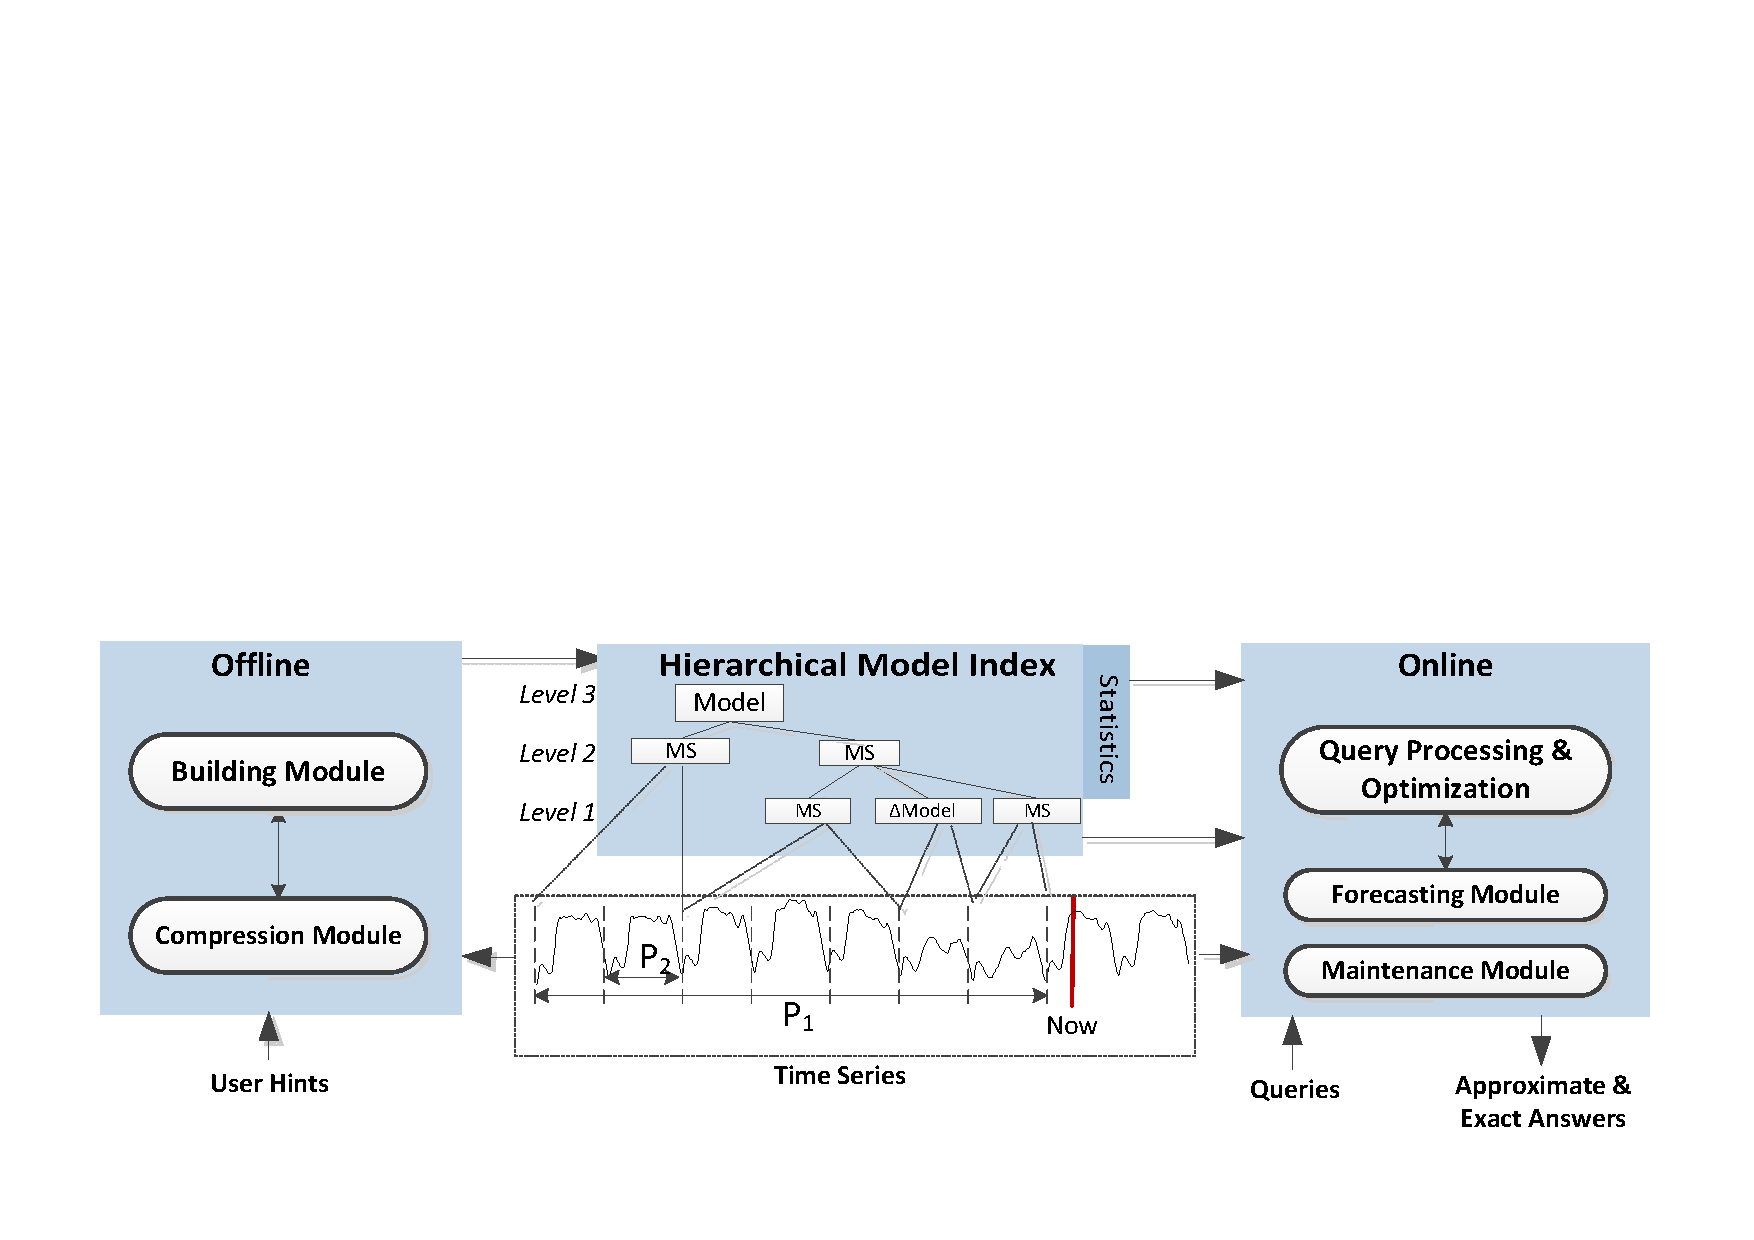
\includegraphics[width=5.5in]{overview5.pdf}

\caption{TimeTravel Overview}
\label{fig:arch}
\end{figure*} 
% As approximate answers can be computed order-of-magnitude faster than their counterpart exact queries. Therefore, our system support computing approximate queries within error guarantees over future and historic data.

We demonstrate TimeTravel, an efficient DBMS system for seamless integrated querying of past and future time series values, supporting two types of queries:
(a)~approximate queries on past and future within user-specified error bounds (i.e., absolute error and confidence), and (b)~exact historic queries. 
We use trend and seasonality to build models over the underlying time series. Here, past and future data is treated similarly, allowing
seamless integrated querying. The main difference of future data compared to past is that the (estimated) error is typically higher.
To organize these models, we introduce a novel index structure, denoted as {\em \LN}.  The upper levels in the index are more ``coarse-grained'', representing 
the underlying time series with a higher error and a lower confidence and fewer model segments compared to the lower levels which are more accurate. 
For approximate historical queries (e.g., last month in our motivating example), we use the highest-level models to calculate an approximate answer. If the  answer 
violates the user requirements on error and confidence, we consult relevant models at lower levels.  We continue traversing the hierarchical model index until either the error guarantee given by user is met or the underlying time series is accessed.
In addition, TimeTravel efficiently answers exact queries by utilizing the index  to find the relevant portions in the time series. 
For example, considering MIN aggregation queries, we only access the
portion of the time series where the minimum value might exist.
For future queries (e.g., next month in our motivating example), we use the model index to retrieve forecast states which is supplemented to  statistical forecast methods.%TODO UNCLEAR 
We meet the user required error guarantees on future data by (a)~controlling the error and confidence of the  retrieved forecast states and (b)~optimizing the forecast method parameters. 

To build the hierarchical model index, the user specifies hints for: (1)~seasonality periods, (2)~error guarantees levels, and (3)~the statistical forecast method (e.g., ARIMA).  
We recursively divide the time series into non-overlapping intervals and build a model on each interval until all error requirements are satisfied. 
Over time, {\it new} values are added to the time series, and we incrementally update the parameters for the forecast method and the hierarchical model index.
%Please note that confidence while building models to reduce the effect of  {\it outliers} on the quality of models.
%For queries on future data, we use  statistical  forecast methods which use states (i.e., past values) and parameters.  Approximate answer,  which usually sufficient for the user, can be computed in order of magnitude faster than their  counterpart exact queries. Our proposed system supports approximate and exact queries. For approximate answer, user specifies error  guarantees on the reported result. 
%i.e., an upper bound on the error, $\epsilon$ and lower bound on confidence $\delta$, i.e.,  Pr ($ans_{approx}$ $\in$  [ $ans-\epsilon$, $ans+\epsilon$]) $>$ $\delta$, where  $ans_{approx}$ and $ans$ are the  approximate and exact answers respectively.

%(2)~expected workload, (3)~error and confidence levels, (4)~the upper bound on the storage size of the index, and (5) the forecast method (e.g., ARIMA).  
% As there are several possible ways to divide the time series,  we introduce a metric denoted as the model utility to find best models. The model utility  is  the speedup on  expected workload with and without this model . 

%In the rest of this paper,   Section~\ref{sec:overview} provides an overview of the our proposed system. Section~\ref{sec:details} describes building the hierarchical model index, and  gives the details of query optimization and processing for approximate and exact queries.  The  related work is presented in Section~\ref{sec:related}. Section~\ref{sec:demo} covers our demonstration scenario  using  real-world time series data.
\section{TimeTravel Overview}
\label{sec:overview}
%The main idea (center down in Figure~\ref{fig:arch}) is to use  a  hierarchical  model structure to facilitate  answering approximate queries and indexing the time series.
%The models at the highest level decompose the time series into three components: trend, seasonality, and error.
Our prototype  system, TimeTravel, is implemented {\em inside} the PostgreSQL database engine.  The user specifies a number of time series and the system builds a separate model index for each. Figure~\ref{fig:arch} illustrates the main modules and data structures of TimeTravel. {Time series} is stored as an array. A time series can have an arbitrary number of seasonality periods (e.g., the shown time series exhibits two seasonality periods $P_1$ and $P_2$). The \LNs is presented in the top center of Figure~\ref{fig:arch}. Each model segment, MS for short, at level $l$ has zero or more children segments at level $l-1$.  Each child segment improves its parent's representation of the underlying time series by building either (a)~a more detailed model over the time series, 
or (b)~models of the error of the parent model. We denote the latter models as $\Delta$Models. 
For query optimization, we store statistics about the index in the system catalog. Specifically, we store the number of model segments, their average size, and the maximum error and minimum confidence for each level. These statistics are needed to estimate the expected cost for the query.
The main modules  can be presented as follow:
%Our proposed system consists of the following modules:
% At level $l$, we represent the underling time series $y$ using one or more models ($M^l_1$,$M^l_2$,$\dots$). The error of model $\epsilon(M)$ over interval $I$ is defined as the $l$-maximum absolute difference between the time series data point $y(t)$ and the modeled value $\hat{y}(t)$, where $l$=(1-$\delta(M)$) * $|I|$, the confidence of the model is $\delta(M)$.  Similarly, we compute the error of level $l$, $\epsilon(M)$. As we traverse down the hierarchy,  the error decreases and the confidence increases. 

% For a  model $M$ at level $l$  in the index, we need to determine the interval  range, the upper bound of the error,  the lower bound of confidence, and  branching factor, i.e., the maximum number of intervals at level $l-1$  that are defined over the same interval range.

%find the ''best'' \LN that minimizes the  run time of expected workload while complying with  the specified  storage overhead.


{\em Building Module.}  The purpose of this  module is to take user hints and time series as inputs, and output a compatible \LN. 
We use heuristics to determine the model parameters. This module is invoked offline and presented in Section~\ref{sec:building}.

   %determines the interval range, error, confidence, and parameters for each model in the index
%the details of processing  of trend, seasonality, and error components. 

%Hence, the search space to find the best models is large.  User gives hints to specify parameters for the index and  time series to  reduce the search space. We introduce a metric denoted as the model utility. The utility model for $m$, $U(m)$, is the  speedup of expected workload using  model $m$ and its children  models is relative to the storage space needed. 

{\em Compression Module.} This module reduces the required storage space for \LNs by finding similar model segments, based on trend and seasonality components, and combining them into fewer segments. % We use  parameters of trend or seasonality to find the similarity between models.   %Section~\ref{sec:compression} gives the details of this module. 


{\em Query Processing Module.} We extend the query processor and optimizer of PostgreSQL to support approximate queries over future and past data and exact queries over the past data. 
To answer historical queries, it traverses down the model index. The Forecasting module is used to retrieve the predicted the time series.
The query processor supports point, range, aggregate, and join queries, as discussed in Section~\ref{sec:online}. 
%For historical queries,  it traverses down the \LN until    the answer meets the user requirement of error guarantee or the underlying time series is  accessed.
%For forecast queries,  we use the forecasting module to retrieve the  predicted the time series.  The forecasting module uses the values of historic data supplied by query processing module and forecast method parameters.

%we use the model at level $n$ ( i.e., the highest level in the hierichy) to obtain an approximate answer for the query. If the answer violates the user requirements of the error and  the confidence, we consult relevant models at level $n-1$ to minimize the error and maximum the confidence.
%If and  using the ranges  of  values retrieved from model index, we can arbitrary shrink the ranges by traversing the hierarchy. 
%For historical queries, we start with the highest level $n$  We continue traversing the in-dex hierarchy until either the user requirement is met oAssume we compute the selWe traverse the hierircal down 

{\em Forecasting Module.} The forecasting module is responsible for: (1)~predicting the values of time series for a given future interval, (2)~estimating the error and the confidence of the 
forecasted values, and (3)~reestimating forecast method parameters. It uses the query processing module to retrieve the forecast method states. The error of the forecasted data~\cite{tBOX76a} depends on (1)~the forecast model and the length of forecast data and, (2)~the confidence interval of the retrieved states. Further details are presented in \cite{FRL12}.
 
% We reduce the error We reduce the We find more accurate approximate ,  we first use query processing module to find more accurate  data of historic values. Then, we  increase the confidence then we 
%The goal of model maintenance is to provide a logicalconsistency between a time series and the models that are based on it. The most expensive part in model maintenance is parameter estimation, since estimators for typical time series models are implemented using numerical procedures and involve optimization algorithms that evaluate complex cost functions many times over all available data of the time series. To address this issue,

%We use the parameters andThe It  by the the  reposnisble for computing the uses the values of historic data supplied by query processing module and forecast model parameters.


{\em Maintenance Module.} 
The Maintenance module maintains \LNs  when new values are added to the time series.
For each level in the index,  we update the last segment (i.e., the rightmost segment in the figure) with the added values. 
If the error and the confidence of the updated segment violates the model error guarantee, we construct a new segment over the interval of the last model and added values, using the building module, and substitute it for the old one. 


%\section{System Details}
%\label{sec:details}
%In this section, we describe the details of building the \LNs for a time series and using this index in query processing and optimization.
\section{The Hierarchical Model Index}
\label{sec:building}
 
% We introduce a  heuristic, $H$,  to  quantify the  {\em goodness} of a model  in fitting a time series over interval $I$. We define the heuristic  $H$  as $(\sum_{\forall e} {|I_e|})/s$, where $|I_e|$ is the length of interval $I_e$ $\in$ $I$ which complies with the error  guarantees $e$, and $s$ is the model size.
 
%  To build the \LN, we  compute the trend $t$, seasonal $s$, and remainder $r$ components for time series $x$. Then, we process each component  as described  in Sections~\ref{sec:nonseasonal}-\ref{sec:error}. We greedy choose the  presentation of model that maximizes the  heuristic $H$. If the LN does not comply with all error guarantee levels,  we  recursively build  models over sub intervals.
 
We now describe how to construct a \LNs over the time series. Initially, we build one model segment over the entire time series. Based on the model error, 
we divide the time series into non-overlapping sub-intervals $I_i$ (e.g., using approaches in \cite{functionDB,Shatkay}). 
The user specifies hints for the seasonal period hierarchy.
For an hourly time series, Figure~\ref{fig:hints} shows two possible hints for seasonality. The first hint should be used if the shape of the time series is similar per year, week and day.  
If the daily shape for weekdays differs from that of weekends, using the second hint reduces the approximation error.
To build model segment $m$ over interval $l$, we first decompose the portion of time series over this interval into {\em trend} $t$, {\em seasonal} $s$, and {\em remainder} $r$ components using the longest seasonal period $p$ in the hierarchy, such that the length of the interval is at least  twice $p$. Then, we process each component as described  later. 
To find the best model representation, we maximize a heuristic, $H$, based on the computed sub-intervals and the size of the model.  Heuristic, $H$, is defined as $(\sum {e_i * |I_i|})/s$, where $|I_i|$ is the length of sub interval $I_i$, $e_i$ is the number of error guarantees levels which complies with interval $I_i$, and $s$ is the model size.

%using  , where $|I_e|$ is the length of interval $I_e$ $\in$ $I$ which complies with the error  guarantees $e$, and $s$ is the model size.
 %in Sections~\ref{sec:nonseasonal}-\ref{sec:error}.
 
{\bf Processing Trend Component}
\label{sec:nonseasonal}
We use  linear Chebyshev regression method~\cite{cheb} to approximate the trend component over the model interval. The Chebyshev regression method is efficiently computable and 
minimizes the largest deviation (i.e. error) from the original curve (i.e., time series) among the polynomials of the same order. 
\begin{figure}
\center
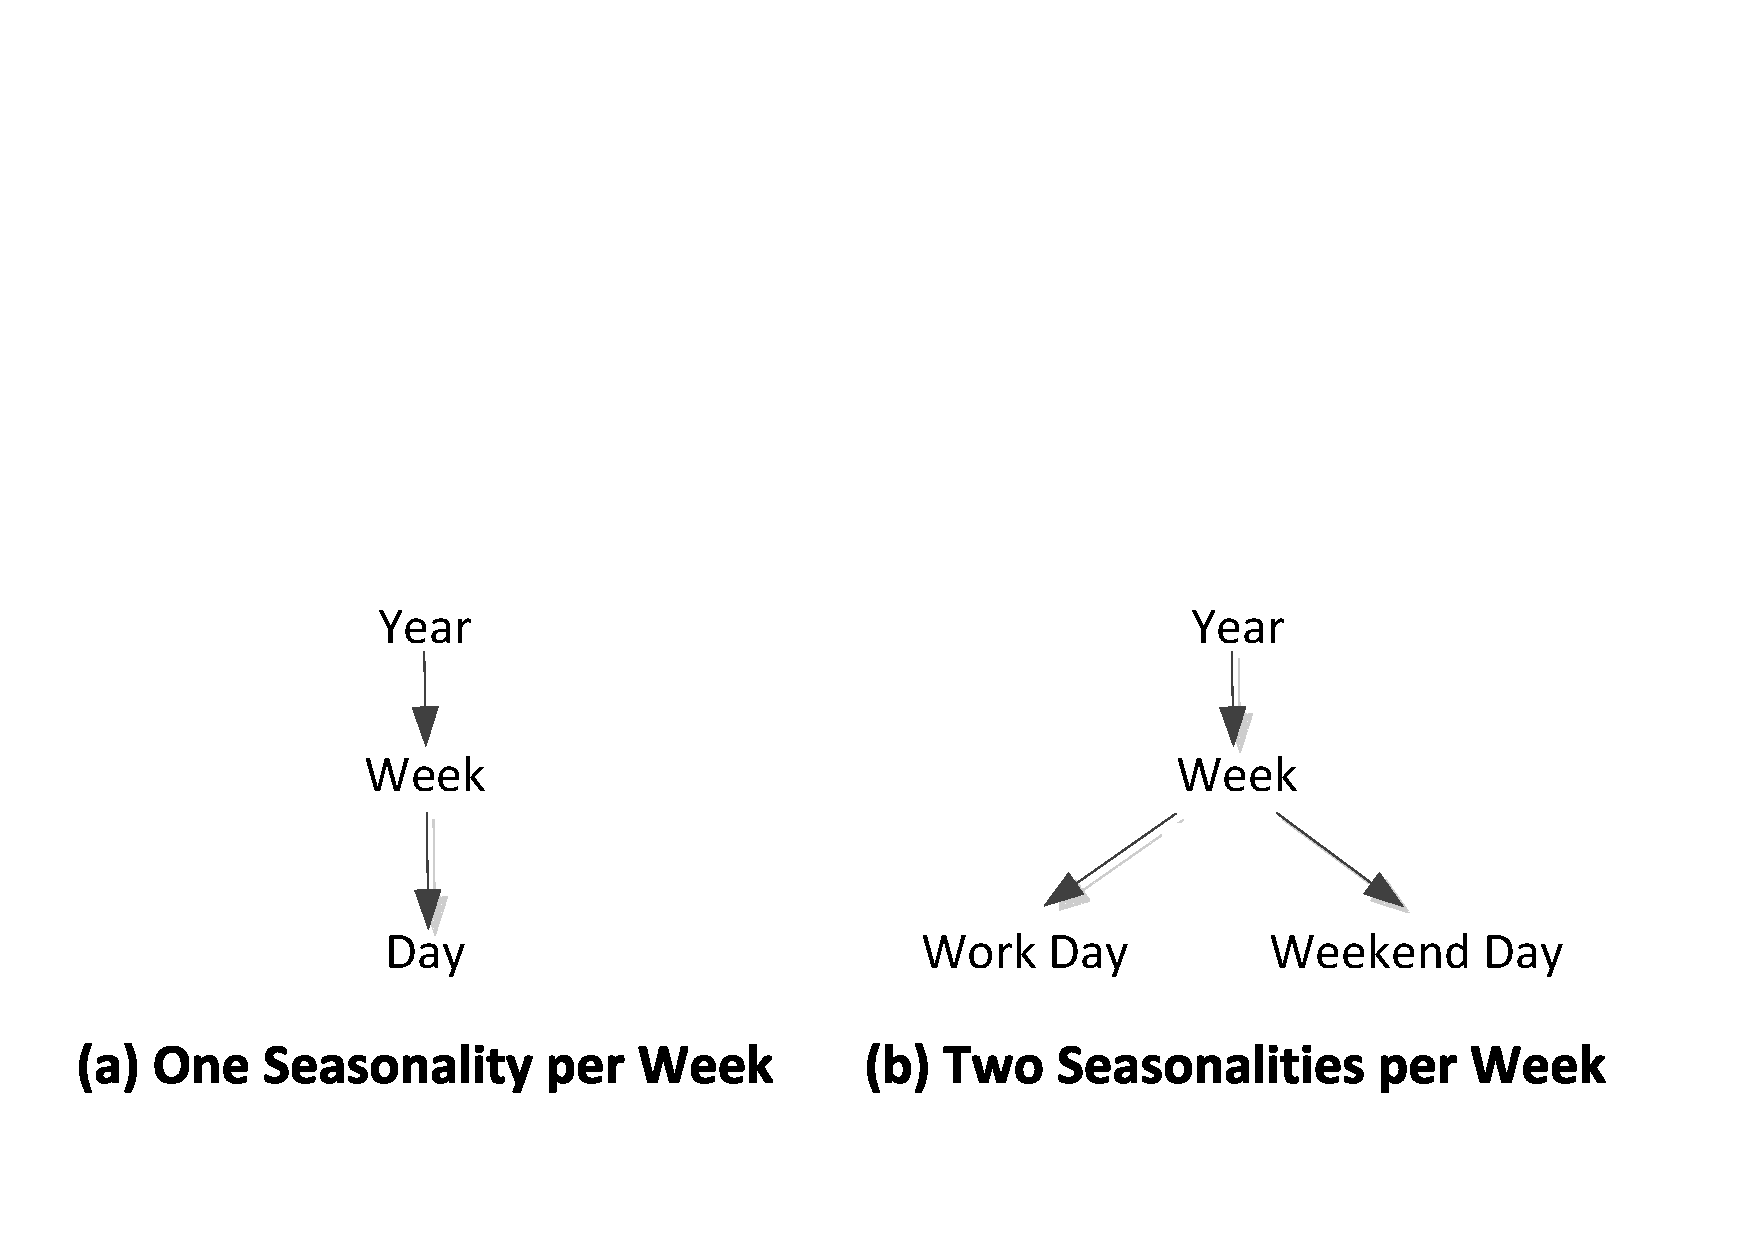
\includegraphics[width=3.0in]{hints.pdf}
\caption{Possible Hints for Seasonal Hierarchy}
\label{fig:hints}
\end{figure}

{\bf  Processing Seasonality Component}
\label{sec:seasonal}
%Trends, seasonality error
We use the hints for seasonality given by the user to efficiently store the seasonality component. 
Storing the value of each data point in the seasonality component may be expensive (e.g., yearly seasonality).  We may approximate the seasonality component using the user hints by 
recursively calculating the trend and seasonality using smaller seasonality periods. 
To find the best approximation for seasonality, we utilize the heuristic described above. 
 
{\bf Processing Error Component}
\label{sec:error}
As regression and seasonality model does not perfectly fit the input time series, errors exists. 
Error is computed as $x$-($\hat{t}$+$\hat{s}$), where $x$ is time series  over interval $I$, and $\hat{t}$ and $\hat{s}$ are the stored model  values for the trend and seasonality components, respectively.
We split the error values into at most $k$ intervals on the time dimensions, where $k$ a system parameter representing the maximum fan-out in the model index. For each interval, we can either (1)~apply a data clipping techniques (e.g., \cite{isax2}), (2)~ store upper and lower error bounds, or (3)~fitting a model (i.e., $\Delta$Model) to the error.  We choose the representation that maximizes the heuristic described�above. 

 %To find best models at each level, we use a heuristic to quantify the  {\em goodness} of model $m$ in fitting the time series $x$. 
 
 %the And find the presentation that maximize the  %Several heuristic (e.g., ~\cite{functionDB} and \cite{Shatkay}) can be used to divide the interval $i$ into sub intervals. including approaches. 
  
 %Let $x$ be  and $\hat{x}$ be the time series and approximation. 
 
%Let the maximum branching factor for models be  $K_{max}$ and the levels of  error guarantees  be ($E$,$\Delta$)=($\epsilon_1$, $\delta_1$), ($\epsilon_2$,  $\delta_2$), $\dots$. 
%We find up to $K_{max}$ intervals $I_1$, $I_2$, $\dots$, such that we maximize $\sum{|I_i|^2\frac{\delta_i}{\epsilon_i}}$, where $|I_i|$ is the the length of  interval $I_i$ and $\exists$ ($\epsilon_i$, $\delta_i$) $\in$ $E\cup(\infty,0)$, s.t. $\delta_i$ and $\epsilon_i$ are the lower and upper  bound of confidence and error of model $m$ on interval $I_i$. 
%If the error and confidence matches the minimum error and maximum confidence in $E$, no further processing is needed.
%Otherwise, we remove from $E$ all error guarantees that are stratified by  model $m$, and recursively build a new model whether error model or  over each intervals.

%new level is needed if the error of the last model does not comply the minimum errro guranteee
%We divide the error into two sets of intervals $I_g$ and $I_l$ for intervals with   error greater and lower than the error $\epsilon$, $I_g$ and $I_l$ respectively. 
%Then, for each intervals in $I_g$, if the difference of the  maximum and  minimum errors in this interval is less than $\epsilon$, we add these intervals to $I_l$.
%Otherwise, we divide each  interval in $I_g$ into two intervals using the point with the maximum error, and add them to $I_g$.
%If the number of intervals in $I_l$ and $I_g$ are greater than $K_{max}$, we repeatly combine adjacent intervals. If the error qurantee of the combined  and compute the error and confidence of the combined interval 

%%{\bf Dividing Interval}. As discussed earlier, we divide interval $I$ if $max(e\in I )-min(e\in I ) > \epsilon$, and the confidence is lower than $\delta$. More specifically, to split an interval $I=(f,l)$, where $s$, $e$ are the first and last index respectively,  into $k$-smaller intervals: 
%%We split  interval $I$ into $k$ intervals $I_1=(f,x_1)$, $I_2=(x_1,x_2)$, $\dots$, and $I_k=(x_{k-1},l)$, such that $x_1$$<$$x_2$$<$$\dots$$x_k$.   Then, we build a model for each interval. The goal is to find $i_1$, $i_2$, $\dots$, $i_k$ which minimizes the total sum of absolute error for each interval.
%each possible represntation and choose the rerepeseantion with the higest
%Basically, er approximate the seasonality using $s$
%Please note model $m$ stores  $\hat{s}$ which approximates the seasonality component $s$.
 %exists within the  seasnoality compoment. over  using smaller periods (e.g., week  build a model  For seasonality period $p$ within interval I over time series $x$, we compute the trend $t(x)$, seasonal $s(x)$, and error $\epsilon(x)$ components.  For trend, seasonality, and error components, we either store or model the values of the component using approaches sections~\ref{},~\ref{} ,~\ref{}, respectively. For  seasonality component, if there is a period $p'$ within period $p$, we recursively  model  the seasonality  with period $p'$, otherwise we use non-seasonality  modeling.
 
% For example, the power usage differs for week day and weekends.

 

%To be able to answer approximate answer within the user-defined error and confidence, these modeling errors should be modeled. The main idea  is  to identify the intervals where absolute error  exceed the user model. For these intervals, we create more detailed models.

%With respect to  error level $\epsilon$ and confidence $\delta$ over the interval $I$, we have three possible cases: (1)~$ max_{i\in I}(e_i) < \epsilon$. In the case, the model fits the time series data, and no further processing is needed. (2)~$max_{i\in I}(e_i)-min_{i\in I}(e_i) < \epsilon$. In the case, we store the  minimum  error, no further computations are needed, or(3)~$max_{i\in I}(e_i)-min_{i\in I}(e_i) > \epsilon$.
%In the case, the span of the error  over interval $I$ exceeds the error level.
%We keep removing the data points with the maximum absolute error from this interval until (a)~the confidence is violated, i.e., the ratio of the remaining points is less than the confidence $\delta$. Hence, we divide the interval $I$ into  smaller intervals and build a model over the points for each one, or (b)~the remaining points satisfy either case~(1) or case~(2). 
%We store the minimum error $min_{i\in I}(e_i)$, and a pointer to the model, if any.


%Figure~\ref{fig:a} shows intervals of error for fitting model over  time series from Figure~\ref{fig:data}. As shown, interval $I_1$ and  $I_2$ has er

%\subsection{Compressing The Model Index}
%\label{sec:compression}
%To reduce the storage requirements for the hierarchical model index, we combine  similar models. Two models are similar if the difference metric between their corresponding trends and seasonality values are within a certain threshold.  More specifically, consider models  $M_a$ ,$M_b$ on interval $I_a$, and $I_b$ respectively. First, we align  intervals $I_a$ and $I_b$ to have the same starting point. Then, we compute a model $M$ using the values of time series data from  intervals $I_a$ and $I_b$ with the time dimensions is shifted. If the error and the confidence of the model $m$ over intervals $I_a$ and $I_b$ within the same error and confidence level for models $M_a$ and $M_b$, we (1) discard models $M_a$ and $M_b$ from the model index. (2) store one copy of $M$, and the time shift values for intervals $I_a$ and $I_b$.
% Please note that we still need to store two different error components for  each model.
%More generally, we store the difference in the 
\section{Query Processing}% \& Optimization}
\label{sec:online}
In this section, we describe query processing and optimization for point, range, aggregate, and join queries over past or future data for approximate and exact queries.
The underlying time series is stored as an array indexed by the time attribute.

To completely incorporate the model index into Postgres, we extend the query optimizer to estimate the expected cost of queries using the proposed model index.  Specifically, we add to the system catalog statistical information for average model size, number of model segments, the span of the seasonality component, 
and the maximum error and minimum confidence for each level in the model index. Moreover, we store  the number of data points of the time series that fits in one page.
By using this information, the query optimizer estimates the cost of executing a query using the model index or directly using the stored time series,
and creates the query plan accordingly.
As mentioned in \cite{ArimaDB}, the dominant cost of forecast queries is re-estimating the forecast model parameters. Unfortunately, the burden of this cost cannot be avoided. 
However, we only reestimate the parameters if necessary\cite{FRL12}, and the cost is amortized over the query workload. For simplicity, we do not include it in our cost model.

The general idea of query processing is to construct an approximation for the time series using the models and the error guarantee. Each value is represented as an 
uncertain range $[v+l,v+u]$, where $v$ is the value from the model, and $l$ and $u$ are the lower and upper bound of the error, respectively.
The approximation can be arbitrarily improved by traversing down the index. An important optimization is that we use the model parameters, span of seasonality, and error to find the relevant portion of the time series. %Moreover, we progressively read the seasonality component (e.g., using year  to further increase the accuracy of the approximation. 
%We   An upper bound cost for computing the value of a  data point using the hierical index model is easy to compute by storing the maximum error and minimum confidence for each level in the hiereicy. Let $n_l$ be the number of the  models at level $l$.

{\bf Point Queries.}
As the underlying time series is stored as an array, we need at least one page access to find the value of the time series for any point in the past, with 0\% error and 100\% confidence,  
while for forecast queries, we access the forecast model parameters and states (i.e., historic values). We estimate the cost of finding the values of the historic data either using the time series or using the index structure.
 
%For a query $Q$ with range $r$ over historic data with maximum error $\epsilon$, minimum confidence $\delta$, 
% we find level $l$ such the the error of $l$ is smaller than or equal to $\epsilon$, and the confidence of $l$ is greater than or equals to $\delta$. The expected cost of  model index at level $i$, $c_i$, equals to  $\frac{r}{R}$*$n_i$, where $R$ is the range of the time series, $n_i$ is the number of models at level $i$. Hence, the expected cost of  query is the total sum from level $n$ to level $i$, i.e., $cost(Q)$=$\sum_i^{n}{c_i}$. While the cost of directly use the time series is  $\frac{r}{b}$, where $b$ is the number of data points of the time series that fits in a page.
 {\bf Range Queries.}
 We use the system catalog statistics to estimate the cost of a range query. We accomplish this by computing an upper bound on the number of model segments in the requested range 
at each level in the model index. While the cost of directly using the time series is  $\frac{r}{b}$, where $b$ is the number of data points per page, and $r$ is the query range.
To compute any future data point for forecast queries,  we need to retrieve the relevant forecast states, i.e., to answer a range query $Q$ in the future, we need to compute range queries over the past to get all states. To this end, we can estimate the expected cost for forecast range queries by either  using the model index  or accessing the underlying time series directly. 
Processing a  range query $Q$ can be presented as follows: we traverse down the  model index, discarding  model segments that do not overlap with the specified range $r$ until we reach level $l$ that matches the user requirements of error and confidence.

%For query optimization, we use the same cost model, as aggregate queries. 
{\bf Aggregate Queries}
The query processing and cost estimation for an aggregate query depends on the type of aggregate function used.
For MIN/MAX aggregates, we use the approximated representation of the time series to  identify  possible intervals (i.e., ranges) within the query range where the  minimum (maximum) may exist, 
discarding most of the range of the query.
For SUM/AVG aggregates,  a nice property of linear regression is that the total sum of the errors equals zero. Hence, while traversing the hierarchical model index, we discard an interval $l$ from further processing, if we encounter a model segment $m$ over interval $l$ that fully overlaps with the range of the query.

{\bf Join Queries.}
For simplicity, we limit our discussion to equi-join queries. 
Joining the time series $x$ and $y$ over the time attribute can be performed as follows: we progressively traverse the indexes for time series $x$ and  $y$. If the error of the combined results exceeds the query requirements, we increase the accuracy of join results by traversing down the index  with the maximum error.
 For joining time series on a value attribute, we build an approximate representation for each time series using the model index.  
For each potential intersection (i.e., join output), we eliminate false positives by traversing down the corresponding model index.

\section{Related Work}
\label{sec:related}

MauveDB~\cite{MauveDB} proposed  querying models using a relational framework for sensor data.  FunctionDB~\cite{functionDB} supports regression functions to represent the data. Queries on these function are processed using an algebraic solver.
Pluse~\cite{pluse} is a continuous stream query `processor that can fit one-dimensional functions. It finds the query results by computing the algebraic solution to systems of equations. It back-propagates the query result to validate the error on the input. In comparison, in TimeTravel, we directly associate the model with error and hence can bound the error of the answers. 
 To answer approximate queries Shatkay~\cite{Shatkay} proposed  an algorithm to fit a curve using a set of lines or Bezier curve while bounding the error.
All of these approaches uses only regression functions. Ignoring  seasonality significantly increases the number of needed regression functions. MauevDB and functionDB do not give any error guarantee, nor support forecast queries. In comparison, TimeTravel supports more powerful functions, seasonality, and error guarantees. 

On the other hand,  ISAX~\cite{isax,isax2} and data clipping~\cite{clipping} approximate the time series by mapping each value in the time series to a value in a much smaller domains (e.g., a domain of two values in~\cite{clipping}). 
Unlike our approach, the error of   depends on the cardinality of the mapped domain and the compression ratio.

\balance
%Pluse proposes  a query inversion to bound the  error of query results which is one 
\section{Demonstration Scenario}
\label{sec:demo}
TimeTravel is based on PostgreSQL and integrates
the different modules described in this paper. Our demonstration
shows building  the \LNs for real-world time series, and the effect of varying the error guarantees on the speed up of approximate and exact queries.
The user specifies the seasonality hierarchy,  error guarantees and the statistical forecast method using a graphical user interface.


% The user can browse the hierarchical index and update model  parameters.  
% We show the scalability of our system, and the speed up for approximate queries and  exact queries using the index.

{\bf Time series} We will use several real-world
datasets to demonstrate our system. We mainly use the UK household power consumption time series and 
Australian  tourist visitors nights.
%. In addition, we provide a real-world time series for the number of cars 
%at a certain intersection and visitor nights for Australian  tourism. 
%will provide , traffic one dataset was obtained from the Tourism Research Australia (http://www.ret.gov.au/tourism/tra/domestic/national/Pages/default.aspx) and consists of observations on the number of visitor nights for the Australian domestic tourism according to different countries and purposes of visit. In addition, we will provide real-world datasets from the energy domain. These datasets pose the challenge of high update intervals and demonstrate the necessity of our lazy maintenance scheme.


\begin{figure}
\center
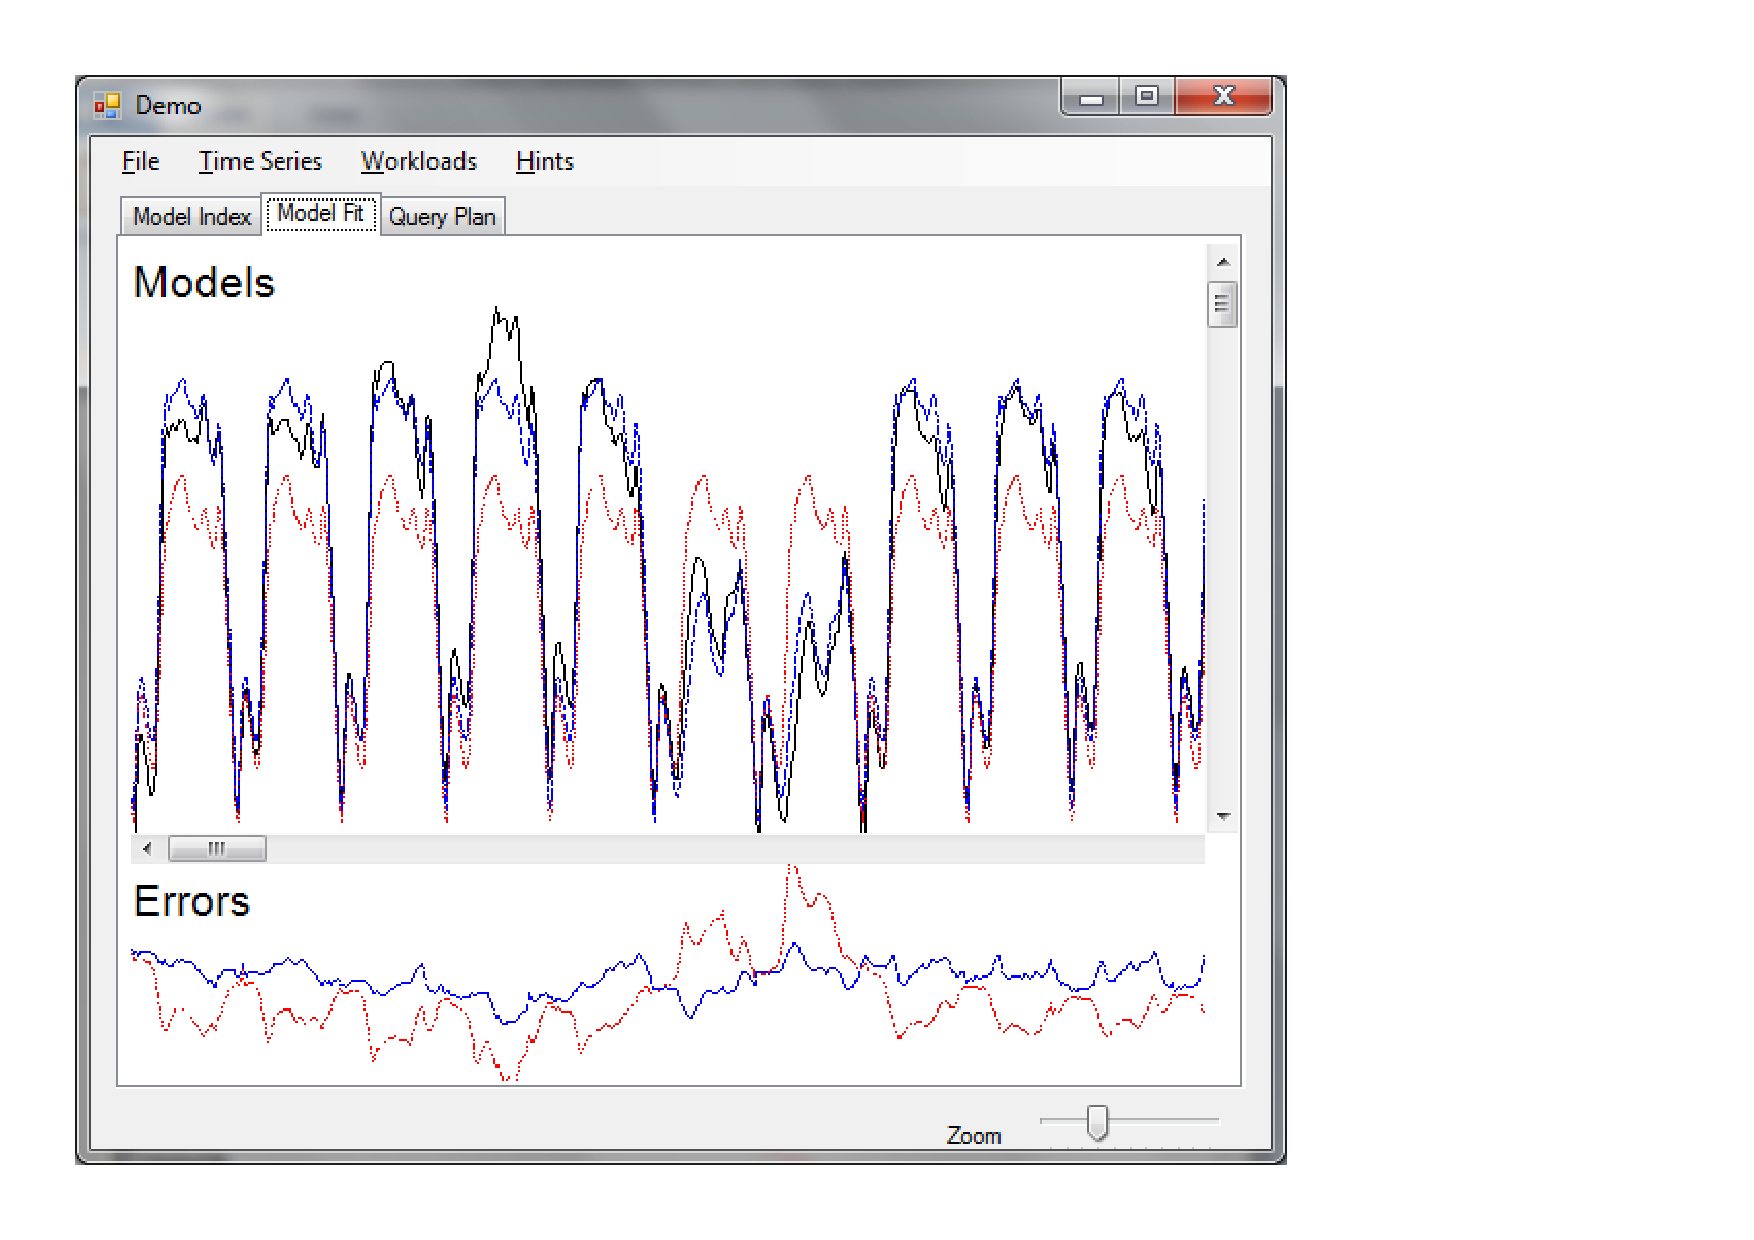
\includegraphics[width=2.8in]{ss1.pdf}
\caption{Model Fit \& Errors for level 1 \& 2}
\label{fig:fit}
%using Seasonality Hierarchy from Fig~\ref{fig:hints} 
\end{figure}
%We canned different configurations to illustrate this effect of changing these values. For each configuration the system computes the expected speed up for the given workload and the storage space needed by the model index.
 
{\bf Scenarios} The prototype is divided in three different
aspects: (1) model index view, (2) model fit view, and (3) query plan view. 
 Using the model index view,  we illustrate building a \LNs using the user hints. A demo user can browse the resulting \LN.  She may change the heuristic function used, or directly update model parameters (e.g., intervals, regression line, or seasonality). The user can interact with  the compression module by combining and separating model segments. For the purpose of the demo, the demo user can submit different query workloads. For any change in the \LN, we estimate the response time for these query workload, as well as, the total storage space.
   
 By using the model fit view, the demo user can investigate how the model fits the time series using different levels of the hierarchy by displaying the models versus the time series and/or plotting the error component.
 Figure~\ref{fig:fit} shows a screenshot of model fit and error using models at level $1$ and $2$. The time series used 
is two weeks from UK household power consumption.  The black line represents the original time series, while the red dashed lines uses model segments at level $2$ which uses the seasonal hint (Figure~\ref{fig:hints}(a)). The blue dotted line shows the models at level 1, which splits the week into workdays and weekend days (Figure~\ref{fig:hints}(b)).
As time passes, we show how the expected future data generated from forecast method fits the actual data, and how updates affect the model index.
 %we can update From a global point of view, a user can view and manipulate the model pool by using our model index (Figure 2). Different workloads can be submitted to our system and statistics like the maintenance cost, forecast accuracy or query throughput can be viewed. This is also an interactive part where the demo visitor can change workloads (e.g., query and insert frequency) and parameters (e.g., model types, maintenance strategy). In addition, we prepared some demo runs in order to benchmark different model configurations (e.g., all possible models vs. advisor recommendation) in terms of average forecast accuracy and query throughput.

Last, we will show the query plan for a set of approximate and exact queries given by the user.  For each query, we show the tradeoff between query cost and the 
error guarantee.


%\section{Conclusion}
%\label{sec:conclusion}
%To acheive that model error, 
%In this paper, we seamlsy integrate historic data and forecasted data. User speci



%Error in forecasted and historic data

%different models paratamer with time (versions of model)

%differnt plans 

%different models on each subset

%use mdoel as an index 

%storing error model

%contexts 


%Future work query optimzer using histogram to ide

% The following two commands are all you need in the
% initial runs of your .tex file to
% produce the bibliography for the citations in your paper.
\bibliographystyle{abbrv}
\bibliography{demo} 
\end{document}
